\documentclass[10pt,a4paper]{article}

\usepackage[margin=14mm]{geometry}
\usepackage{booktabs}
\usepackage{graphicx}
\usepackage{hyperref}
\usepackage{xcolor}
\usepackage{enumitem}
\usepackage{array}
\usepackage{tabularx}
\usepackage{titlesec}
\usepackage{microtype}
\usepackage{amssymb}

\hypersetup{colorlinks=true,linkcolor=black,urlcolor=blue!50!black}
\setlist[itemize]{leftmargin=*,itemsep=0.5pt,topsep=1pt,parsep=0pt}
\setlist[enumerate]{leftmargin=*,itemsep=1.5pt,topsep=2pt,parsep=0pt}
\titleformat{\section}{\normalsize\bfseries}{\thesection}{0.5em}{}
\titlespacing*{\section}{0pt}{0.55em}{0.2em}
\pagestyle{empty}
\setlength{\parskip}{0.2em}
\setlength{\parindent}{0pt}

\newcommand{\defbox}[1]{%
  \noindent
  \fcolorbox{black!55}{black!3}{%
    \begin{minipage}{\dimexpr\textwidth-2\fboxsep-2\fboxrule\relax}
    \small
    #1
    \end{minipage}%
  }%
}

\begin{document}

\begin{center}
{\Large\bfseries Moln\'ar Gate~A3 Meeting Summary}\\[0.2em]
{\normalsize Force--displacement $h$-convergence at $l_c=0.015$\,mm --- supervisor decisions}\\[0.1em]
{\small Analysis revision: \texttt{db4c1fa}\quad$\cdot$\quad No additional simulations are requested at this stage}
\end{center}

\vspace{0.15em}
\noindent\textbf{Purpose:}
(1)~accept H2-PUB as the uniform RF--U reference mesh for later work;
(2)~decide whether matched-state SDV15/crack-path contours are mandatory before the benchmark-reproduction stage, Gate~A3, can be accepted.

\section*{Definitions used in this summary}
\defbox{%
\textbf{Meshes and sizes}
\begin{itemize}
  \item \textbf{H0:} original author-supplied supplementary mesh, with local element size $h\approx 0.00494$\,mm.
  \item \textbf{H1:} intermediate refined mesh, with $h=0.0025$\,mm.
  \item \textbf{H2-PUB:} finest mesh, generated using the publication-reported local resolution $h=0.001$\,mm.
        It uses the published resolution, but not necessarily the exact published mesh topology.
  \item \textbf{$N$:} number of physical finite elements in the model.
        It does not include the additional layered visualization/solution elements.
  \item \textbf{$h$:} local element size in the expected crack-propagation region.
  \item \textbf{$l_c$:} phase-field regularization length scale; here $l_c=0.015$\,mm.
\end{itemize}
\textbf{Quantities and stages}
\begin{itemize}
  \item \textbf{RF2 and U2:} reaction force and prescribed displacement in the loading direction.
  \item \textbf{NRMSE:} normalized root-mean-square difference between two force--displacement curves.
  \item \textbf{SDV15:} phase-field fracture variable, where $0$ represents intact material and $1$ represents fully broken material.
  \item \textbf{Pre-peak:} response before the maximum reaction force.
  \item \textbf{Post-peak:} response after the maximum reaction force.
  \item \textbf{Gate A3:} the project's benchmark-reproduction acceptance gate.
  \item \textbf{MISESERI:} the Abaqus stress-discretization error indicator intended for the later mesh-refinement workflow.
\end{itemize}
}

\section*{Status}
\begin{itemize}
  \item Solvers H0 / H1 / H2-PUB: technical pass\quad$\cdot$\quad RF--U packages complete
  \item Peak / pre-peak $h$-convergence: \textbf{supported}
  \item Post-peak $h$-convergence: \textbf{not fully demonstrated}
  \item Crack-path / SDV15 contours: \textbf{not assessed}
  \item Gate~A3: \textbf{open} --- supervisor decision pending
\end{itemize}

\section*{Mesh family}
\begin{center}
\footnotesize
\begin{tabular}{@{}l r r p{6.6cm}@{}}
\toprule
Mesh & Local element size $h$ [mm] & Physical elements $N$ & Description \\
\midrule
H0 & 0.00494 & 3{,}930 & Original author-supplied supplementary mesh \\
H1 & 0.00250 & 12{,}064 & Intermediate refined mesh \\
H2-PUB & 0.00100 & 33{,}852 & Fine mesh using the publication-reported local resolution \\
\bottomrule
\end{tabular}
\end{center}

\section*{RF--U successive differences}
\begin{center}
\footnotesize
\begin{tabular}{@{}lrrrrr@{}}
\toprule
Pair & $\Delta F_\mathrm{peak}$ & $\Delta U_\mathrm{peak}$ & pre-peak NRMSE & full NRMSE & post-peak NRMSE \\
\midrule
H0$\to$H1 & $4.003\%$ & $5.172\%$ & $0.387\%$ & $21.306\%$ & $62.904\%$ \\
H1$\to$H2-PUB & $\mathbf{0.469\%}$ & $\mathbf{0\%}$ & $\mathbf{0.106\%}$ & $\mathbf{6.011\%}$ & $\mathbf{20.206\%}$ \\
\bottomrule
\end{tabular}
\end{center}

\vspace{0.15em}
\noindent Peak RF2: H0~$0.727608$ · H1~$0.699604$ · H2-PUB~$0.696336$\,kN \quad
$U_\mathrm{peak}$: H0~$0.00610$ · H1/H2~$0.00580$\,mm

\section*{Cost (serial)}
\begin{center}
\begin{tabular}{@{}lrr@{}}
\toprule
Mesh & Walltime & Peak memory (approx.) \\
\midrule
H0 & 00:16:29 & $\sim 0.68$\,GB \\
H1 & 00:46:26 & $\sim 0.91$\,GB \\
H2-PUB & 02:12:38 & $\sim 1.76$\,GB \\
\bottomrule
\end{tabular}
\end{center}
H1 uses about \textbf{35\%} of H2-PUB walltime with nearly the same peak/pre-peak responses.

\section*{RF--U overlay}
\begin{center}
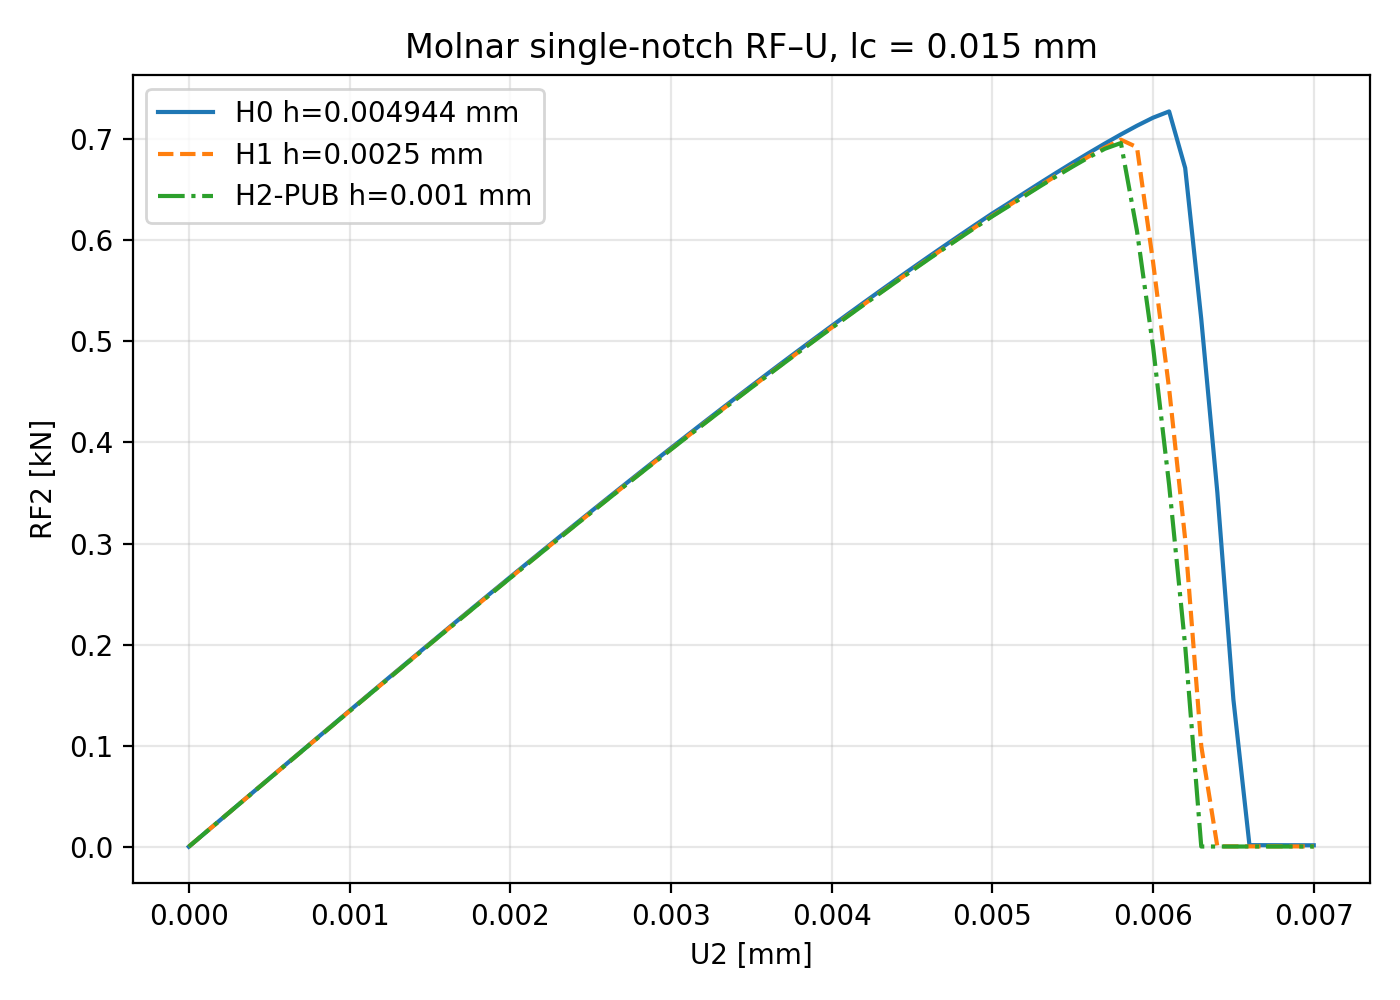
\includegraphics[width=0.88\textwidth]{../../results/figures/molnar_lc015_h_convergence/01_rf_u_h0_h1_h2.png}
\end{center}

\section*{Decisions requested}
\begin{enumerate}[leftmargin=*]
  \item \textbf{Uniform RF--U reference}\\[0.1em]
  $\square$~\textbf{A}~Accept H2-PUB as the uniform RF--U reference\\
  $\square$~\textbf{B}~Accept H2-PUB provisionally (subject to contour evidence)\\
  $\square$~\textbf{C}~Do not accept; specify additional required evidence
  \item \textbf{Contour requirement}\\[0.1em]
  $\square$~\textbf{A}~Contours mandatory before the benchmark-reproduction stage, Gate~A3, can be accepted\\
  $\square$~\textbf{B}~Contours deferred; RF--U evidence sufficient for conditional preparation of the later MISESERI-based mesh-refinement workflow\\
  $\square$~\textbf{C}~Contours required only for H1 and H2-PUB\\
  $\square$~\textbf{D}~Other (please specify)
\end{enumerate}

\section*{Recommended conclusion (project)}
\begin{quote}
\itshape
The intermediate mesh H1 and the fine mesh H2-PUB produce nearly identical elastic, pre-peak and peak-load force--displacement responses.
H2-PUB is recommended as the conservative uniform reference because it uses the publication-reported local crack-path resolution of $h=0.001$\,mm.
H1 may be used for intermediate development studies at lower computational cost.
Noticeable differences remain after peak load, and convergence of the crack path has not yet been assessed.
\end{quote}

\section*{Boundary}
No additional simulations are requested at this stage.
No MISESERI / remeshing / state transfer until Decisions~1 and~2.
A detailed review is available on request.

\end{document}
